\section{Motivation}
As students,
this semester project gives the group a great learning experience as well as a good idea of how such a project would progress.
During the project, the group will learn how to create and setup an Open Platform Communications Unified Architecture, OPC-UA, client,
and how to make it communicate directly to a physical machine.
The group will learn to host a webserver, from which the machine can be controlled,
and access it as a website.
The group will also have the chance to learn and use a new scripting language, JavaScript.
The gained experience is the main motivation of this project.

\section{Aim}
This project aims to offer an interactive web interface for monitoring,
controlling and adjusting the brewery machine. 
This is done by having the web interface interact with a REST API that connects to a client. 
This client controls the machine through an OPC-UA servre connection and stores relevant data in a database.

\section{Solutions}
\begin{figure}[h]
\centering 
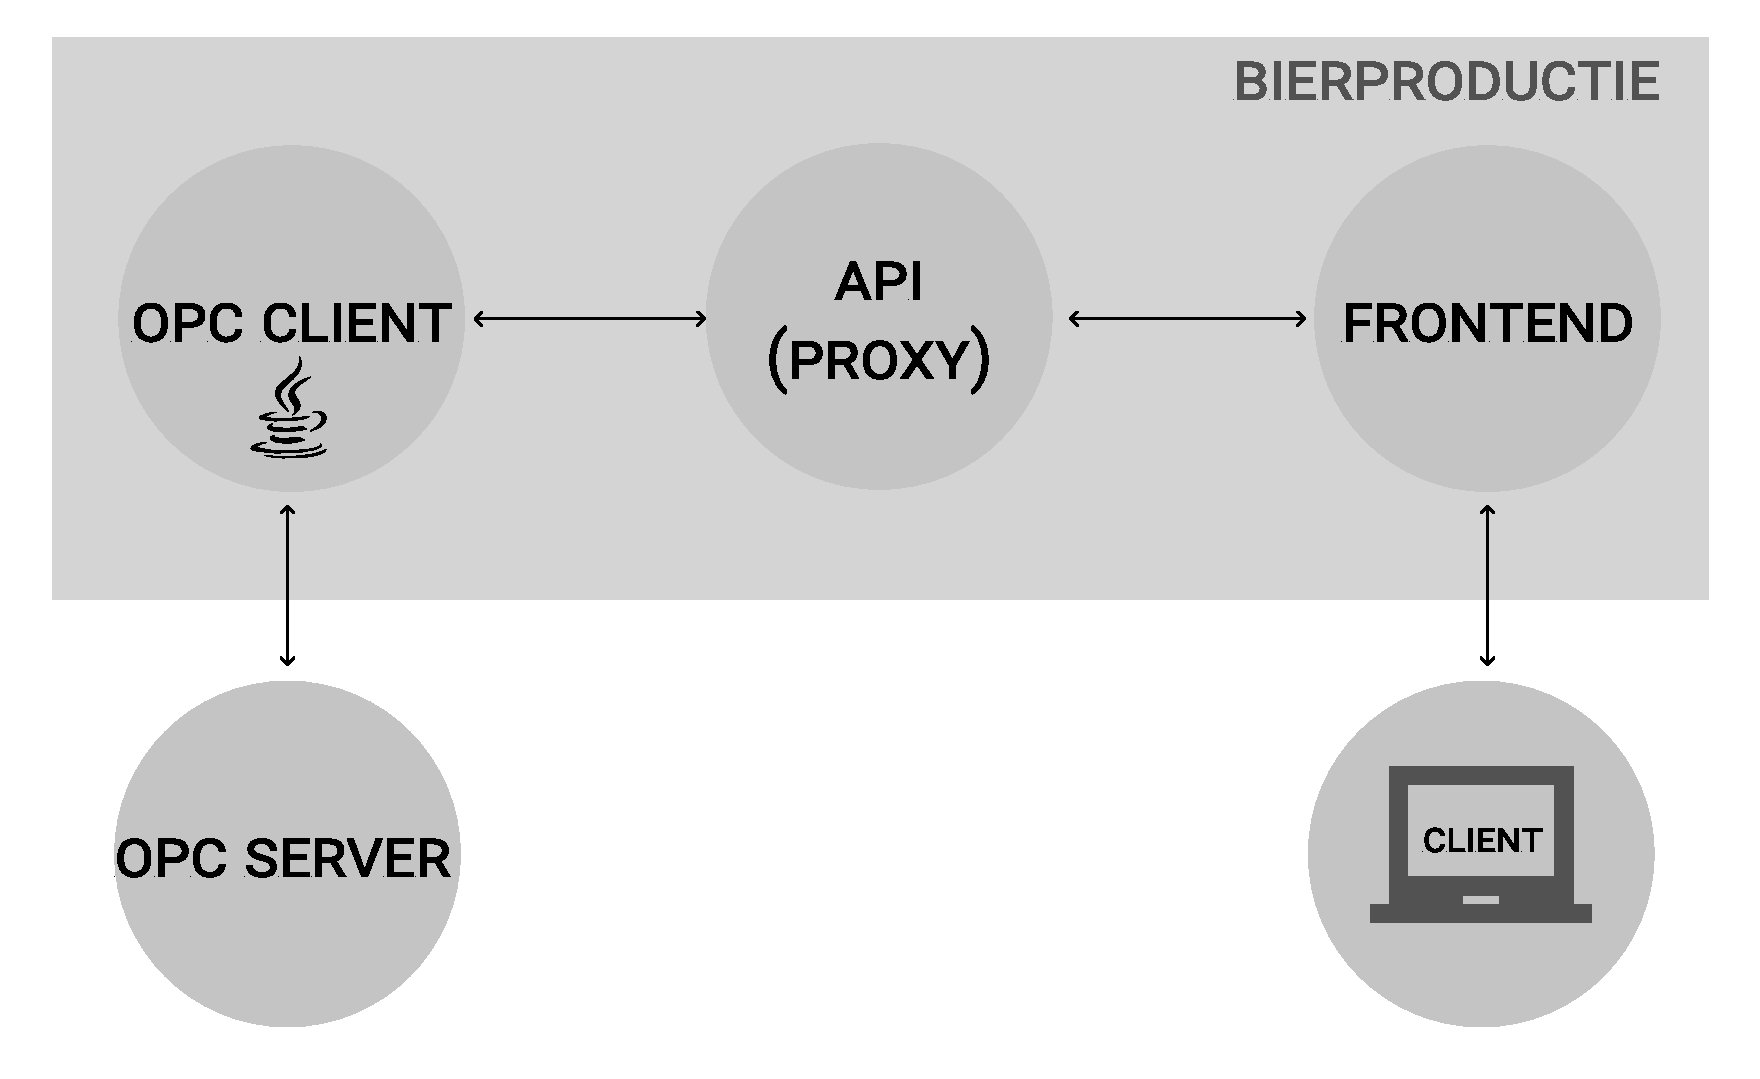
\includegraphics[scale=0.3]{images/system_drawing.pdf}
\label{figure:System_drawing}
\caption{System drawing} 
\end{figure}

The distributed system consists of five sub-systems, where the group are writing three
of them.

\subsection{OPC-UA Client}
The OPC-UA client is responsible for communicating with the brewing machine via
the OPC-UA server. This is needed in order to send and receive data via
commands.

\subsection{Website}
The website user interface is where the client will be able to interface with
our system.

\subsection{REST API}
The REST API functions primarily as a gateway in this design. In order for the
front-end to receive data via fetch calls in JavaScript it needs to talk with
something that speaks HTTP and preferably delivers data in JSON.

\section{Objectives}
The group wants to create a dashboard solution, that gets the necessary
information from the brewery machine to display information about current - and
previous batches.

The group wants to host the REST API and Website on a Linux based server on a
fully qualified domain name using the container technology Docker which should
be configured via Docker Compose. Furthermore the group aims to setup a
continuous integration pipeline for development via GitHub Actions and
continuous delivery via Watchtower.

\section{Methods}
To keep track of the group work the Scrum framework, with a few buts, is used.
Scrum consist of multiple artifacts and ceremonies, and in this project product
roadmap, Scrum meetings, product and sprint backlogs and burndown charts will
be used. Each sprint will have a duration of two weeks and the issues for the
sprint backlog will be chosen at the beginning of each sprint, at the Scrum
meeting. The Scrum meeting will take place each Friday and will be a mixture of
sprint planning, daily Scrum, and sprint review. To manage Scrum, ZenHub, a
management solution that can be integrated with GitHub, is used. On ZenHub the
group will create the roadmap, that acts as a time schedule for the project and
board, which is where the issues will be handled. A burndown chart for each
sprint is automatically generated and kept up to date by ZenHub. The board will
consist of five columns, as seen below.

\begin{table}[H]
    \begin{tabularx}{\textwidth}{|>{\RaggedRight}X|>{\RaggedRight}X|>{\RaggedRight}X|>{\RaggedRight}X|>{\RaggedRight}X|>{\RaggedRight}X|>{\RaggedRight}X|}
        \hline                             
        Product Baklog & Sprint Backlog & In Progress & Review/QA & Closed \\
        \hline
        Issues & Issues for the given sprint & Issues that is currently being worked on & Issues that are pending (or in) review & Approved issues that have been merged    \\
        \hline
    \end{tabularx}
    \caption{Methods} 
    \label{table:Methods}
\end{table} 

\subsection{Tools}
The table below are some of the tools the group are going to need through out
the project. If there is any missing tools not on the list, it will be added.

\begin{itemize}
    \item GitHub
    \item GitHub CI
    \item UAexpert
    \item Mathlab
    \item LaTex
    \item ZenHub
    \item Diverse IDEs and text editors
\end{itemize}

\section{Initial Requirement Analysis}


\subsection{Summary of requirements}
The groups proposed solution will adhere to the requirements given by the brewery Refslevbæk Bryghus A/S.

The manufacturing execution system, MES, must be able to control the brewery’s production.
It must be able to start and stop the production line,
as well as monitor the production and collect data from the production line.
The data must be stored for further analysis.
The MES must be able to keep track of the batches that the new machine is producing,
as well as collect various data from the machine that is associated with the current batch number.
After a finished batch production, the MES must be able to produce a batch report.
The report must contain the following.

\begin{itemize}
    \item This Batch ID
    \item Product type
    \item Amount of products (total, defect and acceptable)
    \item Amount of time used in the different states
    \item Logging of temperature over the production time
    \item Logging of humidity over the production time
\end{itemize}

The MES/SCADA (Supervisory control and data acquisition) system must be able to monitor the production and display live relevant data from the machine.
The documentation of the system must contain an illustration that defines the different components in the setup, in relation to the ISA88\^{}1213 Part 1 Physical Hierarchy model.
The system must have a visualization that can be accessed and used to display the production data.
The system must be able to collect the necessary data from the machine and calculate the overall equipment effectiveness, OEE\^{}131516, of the machine. The OEE must be available to be displayed by the system.
The system must be able to estimate the error function associated with the different products.
The system must be able to find the optimal production speed for each product type, based on an error simulation and the appertaining graph upon which the error simulation is built.

\subsection{List of requirements}
\begin{table}[H]
    \begin{tabularx}{\textwidth}{|>{\RaggedRight}p{1cm}|>{\RaggedRight}p{4cm}|>{\RaggedRight}X|}
        \hline
        \textbf{ID} & \textbf{Name} & \textbf{Description} \\
        \hline
        R01 & Control production line & Start/stop production line \\
        \hline
        R02 & Monitor production & Monitor production (collect data and store said data) \\
        \hline
        R03 & Administer batches & Keep track of batches (batch ID) \\
        \hline
        R04 & Store batch info & Collect various data associated with current batch number from the machine \\
        \hline
        R05 & Batch ID &Collect various data associated with current batch number from the machine \\
        \hline
        R06 & Live data & Monitor and display live relevant data from the machine \\
        \hline
        R07 & Batch report & Produce a batch report (PDF/dashboard style format) \\
        \hline
        R08 & Documentation & Documentation must contain an illustration that defines the different components in the setup in relation to the ISA88\^{}1213 Part 1 Physical Hierarchy model 	\\
        \hline
        R09 & Visualization & Visualization that can be accessed and used to display the production data                                                                                  	\\
        \hline
        R10 & OEE & Collect necessary data from the machine and calculate the OEE. OEE must be available to be displayed by the system                                          	\\
        \hline
        R11 & Estimate error function  	& Estimate the error function associated with the products                                                                                                    	\\
        \hline
        R12 & Optimal Production speed 	& Estimate the optimal production speed for each product type                                                                                                 	\\
        \hline
    \end{tabularx}
    \caption{List of requirements} 
    \label{table:Requirements}
\end{table} 

\subsection{Prioritization of requirements}
The group has decided that at the current state, every requirement is a must have.
A further prioritization of requirements will occur, when the group splits the requirements into issues.

\subsection{Use Case Diagram}
\begin{figure}[H]
\centering 
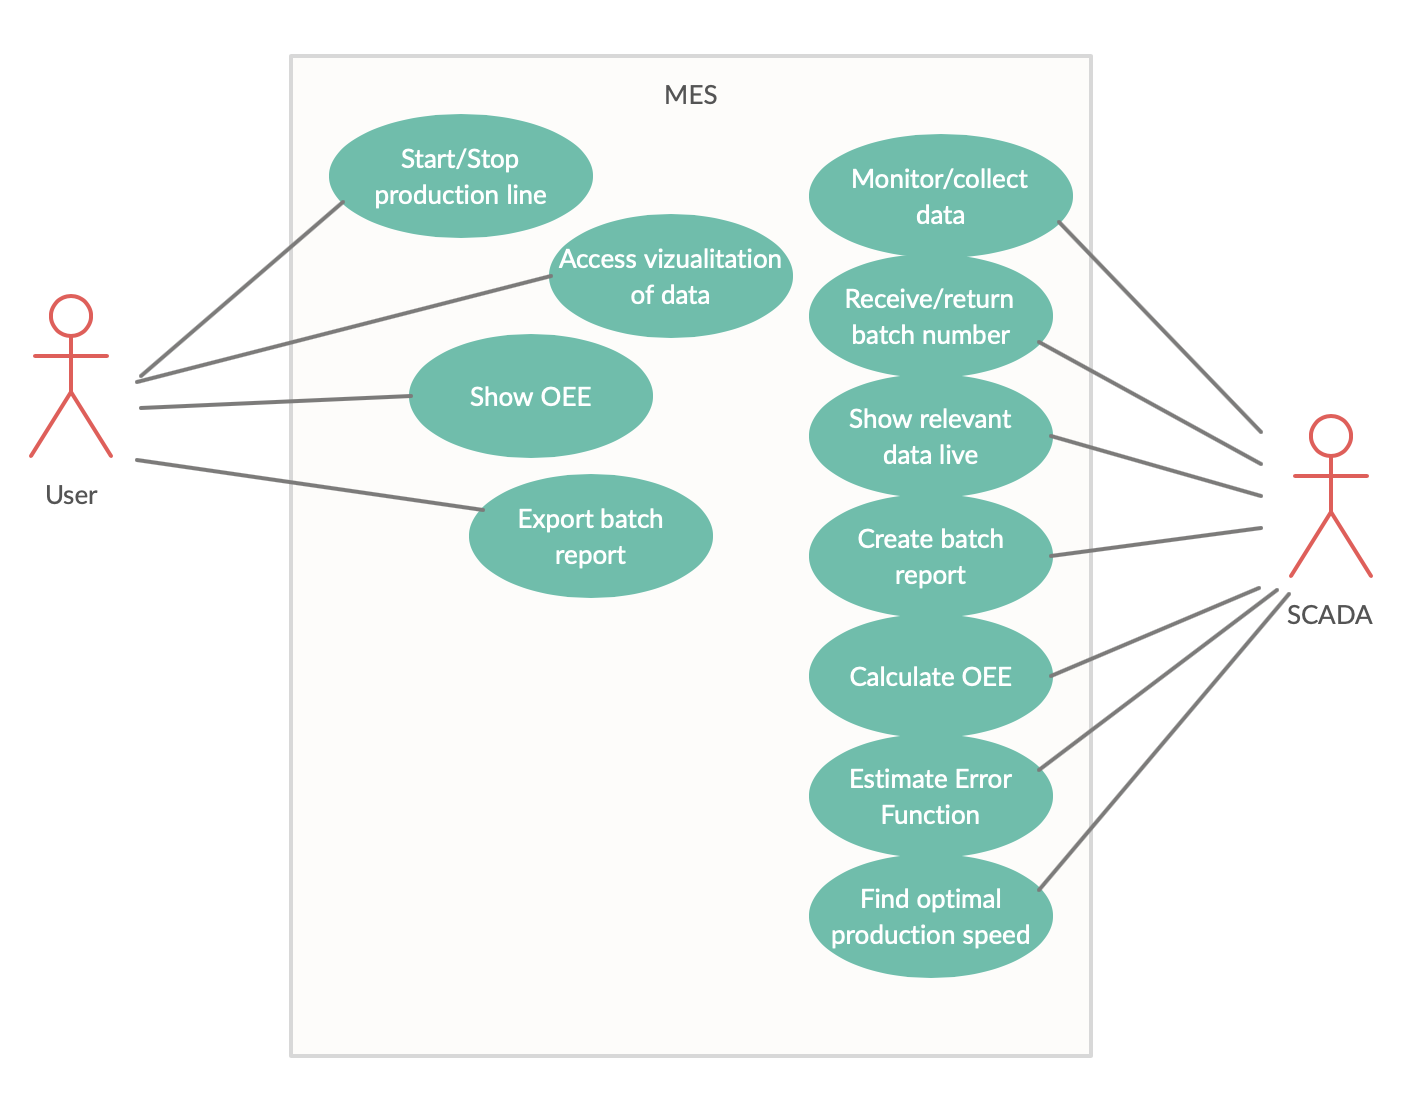
\includegraphics[scale=0.5]{images/ucdiagram.png}
\label{figure:Use_Case_Diagram}
\caption{Use Case Diagram} 
\end{figure}

\subsection{Supplementary Requirements}
\begin{table}[ht]
    \begin{tabularx}{\textwidth}{|>{\RaggedRight}p{4cm}|>{\RaggedRight}X|}
        \hline
        \textbf{FURPS}          	& \textbf{Demands} \\
        \hline
        Functionality  	&  \\
        \hline
        Usability      	& Documentation on usage of the REST API \\
        \hline
        Reliability    	& On server reboot, the application will automatically restart \\
        \hline
        Performance    	& Max response time (API: 400 ms) \\
        \hline
        Supportability 	& Minimum browser versions \\
        \hline
    \end{tabularx}
    \caption{Supplementary Requirements} 
    \label{table:Sup_requirements}
\end{table} 

\section{Stakeholders}
For this project the group does not have any external stakeholders, which is a
problem when developing using SCRUM, since this role is usually filled by a
Product Owner role (abbreviated to PO from here on out). The PO should under
normal circumstances be one from the customers firm, and their job is to choose
which features (user stories) that they would like developed next. Since such a
person does not exist for this project, the group have instead pinpointed
Kristian Nymann Jakobsen to fulfill this role.

\section{Project Organisation}
In this project, work is distributed from planning meetings. These planning
meetings take place at the beginning of each sprint, where the workload is
estimated and distributed across the team members. Kristian Nymann Jakobsen was chosen to be the
Product Owner, so he oversees the “what”, with a focus on value, time to market
etc. Kenneth Munk Christiansen was chosen to be Scrum Master, so he ensures that the Scrum
framework is understood and is used correctly throughout the project. Like the
rest of the group, they are also a part of the Development Team.

\section{Project Plan}
To be sure that it is feasible to complete the project within the designated
time frame, a project plan has been made with inspiration from the
\href{https://docs.google.com/spreadsheets/d/1mZXxgDiwWwWpSyaQmMcafTjvXa2lQriszwTyt-Pf5BA/edit#gid=0}{project plan} supplied by the supervisor.

\begin{figure}[ht]
\centering 
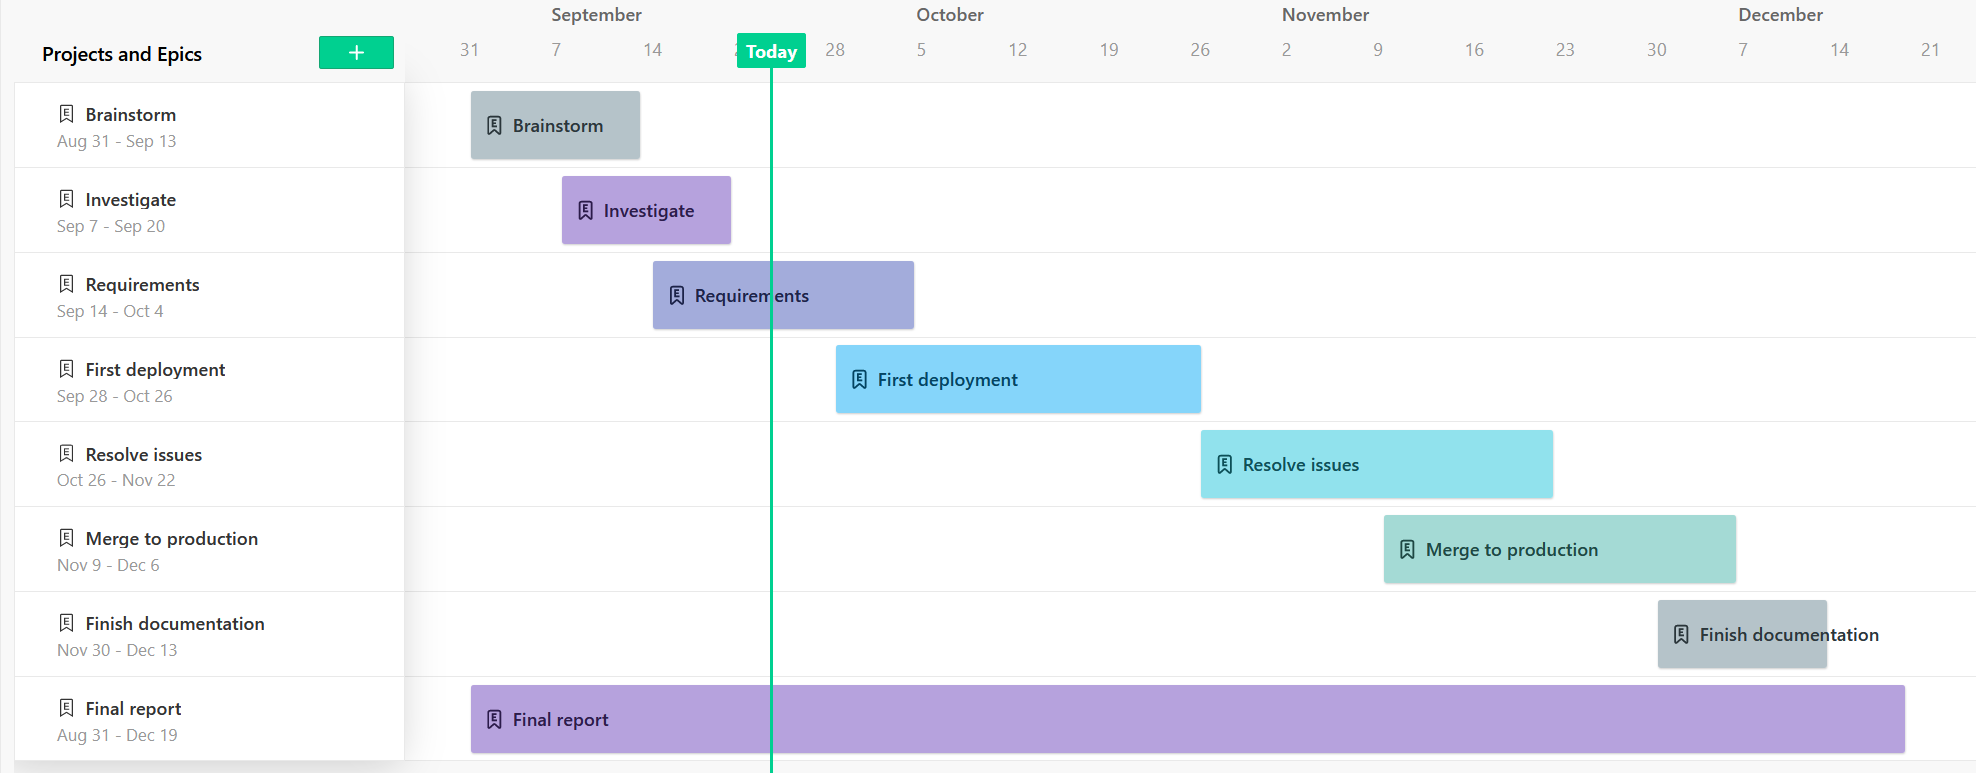
\includegraphics[scale=0.24]{images/roadmap.png}
\label{figure:Project_plan}
\caption{project plan} 
\end{figure}

In this it is shown when the different milestones must be completed to succeed
with the project. As mentioned above, sprints with a duration of two weeks will
be used throughout this project. Each sprint consists of issues from the product
backlog and is chosen at the beginning of each sprint, as described in section
Methods. To keep track of these sprints, a burn down chart will be made, as seen
below.

\begin{figure}[H]
\centering 
\includegraphics[scale=0.3]{images/sprint.png}
\label{figure:Sprint}
\caption{sprint} 
\end{figure}

This ensures the group that each sprint is successfully completed, and if not,
it is easy to see where it went wrong, and the remaining issues can be
transferred to the next sprint.

\section{Risk}
The group foresees three risks with varying impact levels.

\begin{table}[ht]
    \begin{tabularx}{\textwidth}{|>{\RaggedRight}p{1.7cm}|>{\RaggedRight}p{2.2cm}|>{\RaggedRight}p{1.4cm}|>{\RaggedRight}X|>{\RaggedRight}p{1.6cm}|}
        \hline
        \textbf{Risks} & \textbf{Assessment} & \textbf{Impact} & \textbf{Handling} & \textbf{Critical} \\
        \hline
        Covid-19 & High & High & 
        With regulations concerning social distancing and the risk of being infected
        with Covid-19, most work will take place from home. To avoid complications,
        expectations to finish delegated work to each group member will be raised. Each
        member is also expected to follow the lectures. The supervisor will be available
        for contact via e-mail, if questions should arise.
                 & Yes \\
                 \hline
        Schedule & High & High &
        If the group falls behind schedule, the delegated work tasks will be evaluated.
                 & Yes \\
                 \hline
        Lost team member        & Medium & Low & 
        Since the group has already lost a member, the group is currently undermanned.
        To stay on top of the semester project, expectations to finish delegated work to
        each member will be raised.
                                & Yes \\
                                \hline
    \end{tabularx}
    \caption{Risks} 
    \label{table:Risks}
\end{table} 



\section{Milestones}

\subsection{About milestones}
This is our milestones and activities.
\textit{Activities} will include scrum planning and meeting.
It will also show some key activities from the university, that are mandatory
and at last it will also show when the project is need to be handed in.
\textit{Milestones} is the overall structure of the project.
Milestones show the different phases the group will go through.

\begin{table}[H]
    \begin{tabularx}{\textwidth}{|>{\RaggedRight}p{4cm}|>{\RaggedRight}p{5cm}|>{\RaggedRight}X|>{\RaggedRight}X|>{\RaggedRight}p{1cm}|}
        \hline
        \textbf{Phase} & \textbf{Activities} & \textbf{start date} & \textbf{end date}  & \textbf{week} \\
        \hline
        Brainstorm           & Scrum planning (1)       & 28-08-20   &          & 35   \\
        \hline
                             & kickoff                  & 01-09-20   &          & 36   \\
                             \hline
        Investigate          & Scrum meeting            & 04-09-20   &          & 37   \\
        \hline
        Requirements         & Scrum planning (2)       & 11-09-20   &          & 38   \\
        \hline
                             & Scrum meeting            & 18-09-20   &          & 39   \\
                             \hline
        First deployment     & Scrum planning (3)       & 25-09-20   &          & 40   \\
        \hline
                             & Team leader meeting      & 25-09-20   &          &      \\
                             \hline
                             & Project draft            & 02-10-20   &          &      \\
                             \hline
                             & Peer feedback start      & 05-10-20   & 09-10-20 & 41   \\
                             \hline
                             & Scrum planning (4)       & 09-10-20   &          &      \\
                             \hline
                             & Final project foundation & 18-10-20   &          & 42   \\
                             \hline
                             & Scrum planning (5)       & 23-10-20   &          & 43   \\
                             \hline
                             & Team leader meeting      & 09-10-20   &          &      \\
                             \hline
                             & Project week             & 18-10-20   & 24-10-20 &      \\
                             \hline
        Resolve issues       & Scrum meeting            & 30-10-20   &          & 44   \\
        \hline
                             & Code review              & 30-10-20   &          &      \\
                             \hline
                             & Scrum planning (6)       & 06-11-20   &          & 45   \\
                             \hline
                             & Scrum meeting            & 13-11-20   &          & 46   \\
                             \hline
        Merge to production  & Scrum planning (7)       & 20-11-20   &          & 47   \\
        \hline
                             & Scrum meeting            & 27-11-20   &          & 48   \\
                             \hline
        Finish documentation & Scrum planning (8)       & 04-12-20   &          & 49   \\
        \hline
                             & Scrum meeting            & 11-12-20   &          & 50   \\
                             \hline
                             & Scrum meeting            & 18-11-20   &          & 51   \\
                             \hline
                             & Final report             & 02-12-20   &          &      \\
                             \hline
    \end{tabularx}
    \caption{Milestones} 
    \label{table:Milestones}
\end{table} 

\section{Tentativ outline}
The estimated outline of the project report is as follows;

\renewcommand{\labelenumi}{\Roman{enumi}}
\begin{enumerate}
    \item Cover(title, information, signatures)
    \item Summary
    \item Preface
    \item Table of Contents
    \item Editorial(contribution table)
    \item List of figures
\end{enumerate}
\renewcommand{\labelenumi}{\arabic{enumi}}

\subsection{Main report}
\begin{enumerate}
    \item Introduction
        \begin{enumerate}
            \item Motivation?
            \item Problem formulation
        \end{enumerate}
    \item Background
        \begin{enumerate}
            \item Review of relevant literature and other background information
        \end{enumerate}
    \item Problem analysis
        \begin{enumerate}
            \item Use-case analysis
            \item Use-case realization
        \end{enumerate}
    \item Theory and Methods
        \begin{enumerate}
            \item Theory
            \item Methods
        \end{enumerate}
    \item Requirements
        \begin{enumerate}
            \item Overall requirements specification
            \item Selected detailed requirements
            \item Detailed use-cases
            \item Functional and non-function requirements
            \item The physical setup (brewing machine)
            \item Description of the simulator (mathematical?)
        \end{enumerate}
    \item Architecture (System architecture)
    \item Design
        \begin{enumerate}
            \item Description of specific parts of the system (what's important and interesting)
        \end{enumerate}
    \item Implementation (description of technically complicated parts of the system)
    \item Verification and validation (verify, simulate and test that the implemented system fulfils the requirements)
    \item Evaluation (Evaluation of the developed product from a user/customer point of view)
    \item Conclusion
    \item References
    \item Appendix (all technical details that are not essential to understanding the report)
\end{enumerate}
